\section{Maschinelles Lernen}
\setauthor{Lukas Starka}


\section{Deep Learning}
\setauthor{Lukas Starka}


\section{Neuronale Netze}
\setauthor{Lukas Starka}
\subsection{Convolutional Neural Networks}
\setauthor{Lukas Starka}

\subsection{Recurrent Neural Networks}
\setauthor{Lukas Starka}


\section{Text Analysis}
\setauthor{Lukas Starka}

\subsection{Text analysis vs. Text Mining vs. Text Analytics}
\setauthor{Lukas Starka}

Meistens werden die Begriffe Text Analysis und Text Mining im selben Zusammenhang verwendet.
Dabei bedeuten sie eigentlich dasselbe, nämlich, dass man den Sinn einer Nachricht extrahiert.
Deswegen wird in den folgenden Kapiteln nur von Text Analysis gesprochen.

Es gibt jedoch einen Unterschied zwischen Text Analysis und Text Analytics.
Grundsätzlich kann man dabei sagen, dass Text Analysis qualitative Ergebnisse liefert, wohingegen bei Text Analytics die Quantität mehr im Vordergrund steht.\cite{textAnalysisMonkeylearn, machineLearningTextAnalysis}

Bei Text Analysis werden also wichtige Informationen aus der Nachricht herausgelesen.
Oder anders formuliert geht es darum, dass trotz der Unterschiede der menschlichen Sprache trotzdem die Kernaussage herausgefunden werden kann, mit der dann gearbeitet wird.
Es können also dann Informationen herausgefiltert werden, wie beispielsweise, ob etwas positiv oder negativ ist oder was das Hauptthema des Textes ist.\cite{textAnalysisMonkeylearn, machineLearningTextAnalysis}

Auf der anderen Seite wird bei Text Analytics werden verschiedene Muster aus einer großen Menge an Nachrichten herausgefiltert, welche dann in Graphen, Tabellen oder Berichten gezeigt werden können.
Bei Text Analytics geht es also darum Muster und Entwicklungen von numerischen Ergebnissen herauszufinden, bei denen dann Informationen herausgefiltert werden können, wie beispielsweise, die Prozentzahl der positiven Bewertungen.\cite{textAnalysisMonkeylearn, machineLearningTextAnalysis}

\subsection{Warum Text Analysis?}
\setauthor{Lukas Starka}

Im Gegensatz zum manuellen Aufbereiten von Texten sorgt Machine Learning für eine schnelle Bearbeitung, die außerdem auch kostengünstiger ist, weil viele Stellen wegfallen, die benötigt werden würden, um die Texte selber aufzubereiten.
Durch die Verwendung von Text Analysis spart man sich viele Arbeitskräfte, die bei anderen wichtigen Aufgaben innerhalb eines Unternehmens eingesetzt werden können.
Außerdem können dadurch Texte rund um die Uhr und zur Echtzeit bearbeitet werden.
Durch Algorithmen werden außerdem Fehler reduziert, die bei manuellem Bearbeiten leicht auftreten können und Daten können genauer aufbereitet werden.\cite{textAnalysisMonkeylearn}

\subsection{Machine Learning mit Text Analysis}
\setauthor{Lukas Starka}

Grob kann man behaupten, dass ein Text Analysis Tool aus drei verschiedenen Schritten besteht.

\begin{enumerate}
    \item Zunächst muss man sich überlegen, welche Daten gesammelt werden sollen, um damit sein Modell zu trainieren und zu testen.
    Man unterscheidet hierbei zwischen \textbf{Internal Data} und \textbf{External Data}.
    Unter External Data werden Quellen, wie Zeitungen oder Foren bezeichnet und zu der Internal Data zählen sämtliche Daten, die eine Firma jeden Tag generiert, wie E-Mails, Reports, Chats oder Umfragen.
    \item Danach müssen die Daten vorbereitet werden, damit das Programm diese versteht.
    Dieser Schritt wird meistens als \textbf{Data Preprocessing} bezeichnet.
    \item Zum Schluss wird dann ein Machine Learning Algorithmus hinzugefügt, welcher sich um die Analyse kümmert.
    Diesen kann man entweder komplett selber implementieren oder man nimmt sich Libraries zur Hilfe.\cite{machineLearningTextAnalysis}
\end{enumerate}

\section{Natural Language Processing (NLP)}
\setauthor{Lukas Starka}

Natural Language Processing, oft auch als Akronym \textbf{NLP} abgekürzt, sorgt dafür, dass Computer Text auf dieselbe Art und Weise verstehen, wie wir es als Menschen tun.
NLP vereint dabei die Modellierung der menschlichen Sprache mit statistischen Machine Learning und Deep Learning Modellen.
Dies ermöglicht der Maschine im Endeffekt, dass diese menschliche Sprache in Form von Text- oder Sprachdaten zu verarbeiten und sozusagen die komplette Bedeutung und Absicht der Benutzerin oder des Benutzers zu verstehen.\cite{naturalLanguageProcessingIBM}

\subsection{Corpus}
\setauthor{Lukas Starka}

Unter dem Corpus werden die Daten bezeichnet, die verwendet werden, um das NLP Modell zu trainieren, damit dieses menschliche Sprache versteht und damit arbeiten kann.
Der Textkorpus ist also eine Menge von strukturierten Texten, die für den Computer lesbar sind.\cite{corpus}


\subsection{Tokenization}
\setauthor{Lukas Starka}

Bei der Tokenization repräsentiert jeder Token eine sinnvolle Einheit.
Darunter versteht man Wörter, Zeichen oder Sonderzeichen, die alle einen eigenen Token darstellen, lediglich Leerzeichen in einem Satz stellen keine eigenen Token dar.\cite{machineLearningTextAnalysis, naturalLanguageProcessing}

Die verschiedenen Token, die dabei entstehen, können dabei wie in Listing ~\ref{lst:tokenization} aussehen:

\begin{lstlisting}[label={lst:tokenization},caption={Beispiel für die Tokenization}]{Tokenization}
Let us go to the park.

0: Let
1: us
2: go
3: to
4: the
5: park
6: .
\end{lstlisting}

Die Tokenization ist dabei besonders für verschiedene Sprachen von Vorteil, da es in diesen immer andere Regeln gibt, wie die Wörter aufgeteilt werden können.
In dem Beispiel ~\ref{lst:tokenization} wirkt es womöglich so, als könnte man mit einer \textbf{split()} Methode das selbe Resultat erzielen, aber es gibt auch Besonderheiten einer Sprache, die vom Tokenizer bedacht werden müssen, wie folgendes Beispiel aufzeigt.\cite{machineLearningTextAnalysis, naturalLanguageProcessing}

\begin{lstlisting}[label={lst:tokenization-exception},caption={Ausnahme für bestimmte Tokens}]{Tokenization-Exception}
"Let's go to the U.K.!"

0: "
1: Let
2: 's
3: go
4: to
5: the
6: U.K.
7: !
8: "
\end{lstlisting}

\subsection{Part-of-speech-Tagging (POS-Tagging)}
\setauthor{Lukas Starka}

Beim Part-of-speech-Tagging geht es um das Taggen von Wörtern und deren zugehörigen Teil der Sprache.
Als Teil einer Sprache, also dem Part-of-speech, werden grundsätzlich Wörter bezeichnet, die ähnliche grammatikalische Eigenschaften oder Nutzungen besitzen.
Im deutschen sind hierbei also die verschiedenen Wortarten gemeint.

Beim Tagging werden entweder Statistiken angewendet, wie beispielsweise, dass es sehr wahrscheinlich ist, dass nach einem Artikel ein Nomen folgt.
Außerdem gibt es sogenannte Rule-Based POS-Taggers, deren Aufgabe es ist, vordefinierte Regeln zu verwenden, um das Tagging zu vollziehen.\cite{machineLearningTextAnalysis, naturalLanguageProcessing}

Ein Beispiel für POS-Tagging könnte also wie in Listing ~\ref{lst:pos-tagging} aussehen:

\begin{lstlisting}[label={lst:pos-tagging},caption={Beispiel für POS-Tagging}]{POS-Tagging}
I am going to the U.K.

I: Pronoun
am: Verb
going: Verb
to: Part
the: Article
U.K.: Noun
\end{lstlisting}

\subsection{Named-entity recognition (NER)}
\setauthor{Lukas Starka}

Named-entity recognition ist eine der wichtigsten Säulen von Natural Language Processing.
Entities sind strukturierte Stücke von Informationen, die sich innerhalb der Nachricht einer Benutzerin oder eines Benutzers befinden.
Dabei werden Entities aus Texten erkannt und anschließend mit einem Tag der zugehörigen Kategorie versehen.\cite{namedEntityRecognition}

Beispiele für Entities wären also:

\begin{lstlisting}[label={lst:ner-tagging},caption={Beispiele für Enitites}]{NER-Tagging}
PERSON      Personen (inklusive fiktionalen Personen)
NORP        Nationalitäten oder religiöse oder politische Gruppen
FACILITY    Gebäude, Flughäfen, Brücken, Straßen
LOC         Orte
PRODUCT     Objekte, Fahrzeuge, Essen
LANGUAGE    Sprachen
\end{lstlisting}

\subsection{Stemming}
\setauthor{Lukas Starka}

Beim Preprocessing von Texten sind außerdem das Stemming und die Lemmatization Schritte, die häufig durchgeführt werden.

Beim Stemming wird der Wortstamm eines Tokens von den Präfixen und Suffixen gelöst.
Unter einem Präfix versteht man eine Vorsilbe, die dem Wortstamm vorangestellt wird und bei dem Suffix, handelt es sich im Gegenzug dazu um Worterweiterungen, die dem Stamm folgen.
Hierbei gibt es wieder die Möglichkeit selber einen Stemmer zu implementieren oder bereits vorgefertigte Stemmer zu verwenden.\cite{textAnalysisMonkeylearn, machineLearningTextAnalysis}

Ein Beispiel für Stemming von deutschen Wörtern wäre also in Listing ~\ref{lst:stemming} zu sehen.

\begin{lstlisting}[label={lst:stemming},caption={Stemming von deutschen Wörtern}]{Stemming}

verarbeiten ---> ver + arbeit + en
ver             prefix
arbeit          base word
en              suffix
\end{lstlisting}

\subsection{Lemmatization}
\setauthor{Lukas Starka}

Unter der Lemmatization oder auch Lemmatisierung wird der Prozess verstanden, bei dem alle verschiedenen Arten von einem Wort zu ihrem Wortstamm umgeformt werden.

Die Lemmatisierung ist sozusagen eine Weiterentwicklung des Stemming und versucht im Gegensatz zum Stemming den Kontext zu den Wörtern zu bringen.
Je nachdem in welchem Kontext die Verben gebraucht werden können sie sich dabei von ihrer Wortart unterscheiden und so eine andere Bedeutung haben.
Generell lässt sich sagen, dass Stemmer meist einfacher zu implementieren sind und für schnellere Laufzeiten sorgen, allerdings wird von vielen auch die Lemmatization dem Stemming vorgezogen, aufgrund der Vorteile die das Einbeziehen des Kontextes mit sich bringt.\cite{machineLearningTextAnalysis, textAnalysisMonkeylearn, stemmingLemmatization}


Beispiele für die Lemmatisierung sind:

\begin{lstlisting}[label={lst:lemmatization},caption={Lemmatisierung von deutschen Wörtern}]{Lemmatization}
Gut ---> gut
besser ---> gut
las ---> lesen
gelesen ---> lesen
lesend ---> lesen
mag ---> mögen

\end{lstlisting}

\subsection{Parsing}
\setauthor{Lukas Starka}

Parsing könnte man so beschreiben, dass es eine Art ist um einen Satz auseinanderzuteilen, um die Struktur des Satzes besser zu verstehen.
Beim Parsing wird also die syntaktische Struktur eines Textes bestimmt.
Um dies zu erreichen, nimmt der Parsing Algorithmus die Eigenheiten der Grammatik, von der jeweiligen Sprache, in der der Text geschrieben ist, her.\cite{textAnalysisMonkeylearn}

Es gibt zwei verschiedene Arten von Parsing.
Diese sind das sogenannte \textbf{Dependency Parsing} und das sogenannte \textbf{Constituency Parsing}.

\subsubsection{Dependency Parsing}
\setauthor{Lukas Starka}

Beim Dependency Parsing wird die grammatische Struktur eines Satzes bestimmt.
Außerdem kann man mithilfe des Dependency Parsing herausfinden, welche Wörter zusammenhängen und welche Beziehung diese zueinander aufweisen.
Dies bedeutet beispielsweise, dass man bei den Wörtern \texttt{blauer Ball}, \texttt{nette Frau} oder ähnlichem erkennen kann, dass sich die Wörter \texttt{blau} oder \texttt{nett} auf das nachfolgende Wort bezieht.
Ein anderes Beispiel könnten die Wörter \texttt{black} und \texttt{car} sein.

\begin{figure}[hbt!]
    \centering
    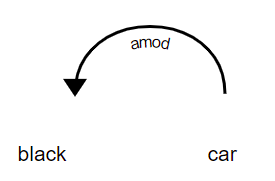
\includegraphics[scale=1]{pics/dependency_parsing}
    \caption{Beispiel für die Beziehung zweier Wörter beim Dependency Parsing~\cite{dependencyParsing}}
    \label{fig:dependency_parsing_relation}
\end{figure}

Wie man aus der Grafik ~\ref{fig:dependency_parsing_relation} entnehmen kann, bezieht sich die Farbe Schwarz in diesem Fall auf das Auto.
Im Englischen wird das Wort \texttt{car} deswegen auch als \textbf{Head} bezeichnet und \texttt{black} ist ein \textbf{Child}, also ein Wort, dass abhängig von diesem \textbf{Head} ist.
Die Beziehung, die zwischen diesen Wörtern vorliegt, wird mit \texttt{amod} bezeichnet.
Dies ist eine Abkürzung für \textbf{Adjectival Modifier}, also ein Adjektiv, welches ein Nomen modifiziert und zu der Bedeutung des Nomens beiträgt.
In diesem Fall gibt dieses eine genaue Beschreibung der Farbe des Autos.\cite{dependencyParsing}

Diese Beziehungen kann man auch in einem Tree darstellen.

\begin{figure}[hbt!]
    \centering
    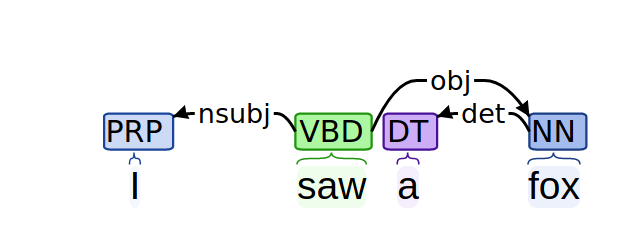
\includegraphics[scale=0.5]{pics/dependency_parse_tree}
    \caption{Darstellung des Dependency Parsing~\cite{dependencyVsConstituencyParsing}}
    \label{fig:dependency_parsing_tree}
\end{figure}

\subsubsection{Constituency Parsing}
\setauthor{Lukas Starka}

Beim Constituency Parsing wird ein Satz in mehrere Teilphrasen zerteilt, die auch \textbf{Constituents} genannt werden.
Im Gegensatz zum Dependency Parsing, bei dem man Beziehungen zwischen den Wörtern innerhalb eines Satzes bekommt, kann man hierbei also die Sätze gruppieren.
Dies kann helfen, um die Struktur von Sätzen aufzuzeigen.
Der Nachteil hierbei ist, dass man nun keinen Context in den Sätzen mehr hat, dafür kann man aber beispielsweise gut überprüfen, ob ein Satz grammatikalisch korrekt oder inkorrekt ist.\cite{machineLearningTextAnalysis}

Die berühmtesten Tags um Constituents zu bezeichnen sind:

\begin{itemize}
    \item VP für Verbalphrasen (Verb Phrases)
    \item NP für Nominalphrasen (Noun Phrases)
\end{itemize}

Der Satz \texttt{I saw a fox} wird hierbei als Tree des Constituency Parsings dargestellt.

\begin{figure}[hbt!]
    \centering
    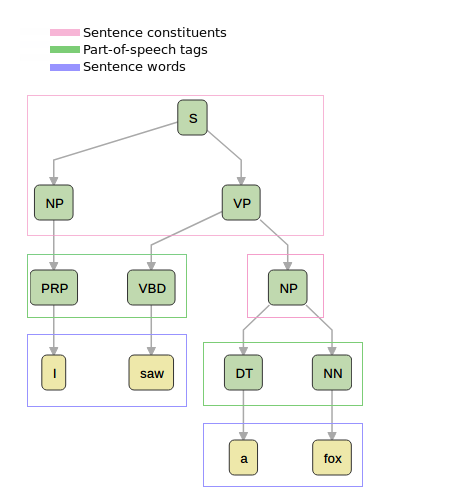
\includegraphics[scale=0.5]{pics/constituency_parse_tree}
    \caption{Darstellung des Constituency Parsing~\cite{dependencyVsConstituencyParsing}}
    \label{fig:constituency_parsing_tree}
\end{figure}

In dem Beispiel ~\ref{fig:constituency_parsing_tree} kann man sehen, dass der Satz in zwei Teile aufgeteilt wurde.
Der Textbaustein \texttt{I} wurde als Substantiv (NP) erkannt und \texttt{saw a fox} ist hierbei die Phrase des Verbs (VP).
Darunter sieht man die Regeln, die dazu führten, dass hierbei erkannt wurde, dass es sich um eine Nominalphrase und eine Verbalphrase handelt.
Diese Regeln werden durch die Grammatik der Sprache erstellt und so sagt beispielsweise die Regel \texttt{S → NPVP} aus, dass ein ganzer Satz (S) durch eine Nominalphrase (NP) und eine Verbalphrase (VP) entsteht.\cite{dependencyVsConstituencyParsing}

\subsection{Stopwords}
\setauthor{Lukas Starka}

Unter Stopwords oder Stoppwörtern werden Wörter verstanden, die häufig in einem Satz vorkommen, aber nicht wirklich zum Informationsgehalt des Textes beitragen.
Deswegen werden diese oft nicht beachtet, da sie keine Relevanz für die Bedeutung des Satzes haben.

Bei den Stoppwörtern handelt es sich meistens um die am häufigsten vorkommenden Wörter einer Sprache.
Deutsche Stoppwörter sind zum Beispiel:\cite{germanStopwords}

\begin{itemize}
    \item was
    \item aber
    \item auch
    \item der
    \item die
    \item das
    \item du
    \item wir
    \item ihr
    \item können
    \item müssen
    \item dürfen
\end{itemize}

\subsection{Vectorization}
\setauthor{Lukas Starka}

Durch Machine Learning können Systeme basierend auf vorherigen Eingaben und Mustern Dinge voraussagen.
Diese Systeme benötigen allerdings Trainingsdaten, um ihre Präzision dabei zu steigern.
Wenn man nun also ein System trainieren möchte benötigt man eine Darstellungsform, die auch von Maschinen verstanden werden kann.
Hierbei kommen nun Vektoren zum Einsatz, weil das System dadurch die wichtigsten Informationen extrahieren und daraus lernen kann.

\subsection{Skalarprodukt}
\setauthor{Lukas Starka}

Beim Natural Language Processing benötigt man sehr oft das sogenannte Skalarprodukt. Dieses kann auch als inneres Produkt oder Punktprodukt bezeichnet werden.
Das Skalarprodukt ordnet zwei Vektoren eine Zahl zu.
Ein Skalarprodukt berechnet man wie in ~\ref{fig:dot-product} zu sehen ist.

\begin{figure}[hbt!]
    \centering
    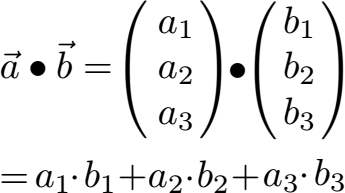
\includegraphics[scale=0.5]{pics/dot-product}
    \caption{Skalarprodukt von zwei Vektoren~\cite{dotProduct}}
    \label{fig:dot-product}
\end{figure}

\subsection{Bag of Words}
\setauthor{Lukas Starka}

Eine der einfachsten Techniken um einen Text nummerisch zu repräsentieren, ist mithilfe der sogenannten Bag of Words Vectorization.
Dabei wird zunächst jedes Wort, welches im Corpus vorkommt als sogenanntes Vokabular gespeichert.
Danach wird in jedem Satz die Anzahl dargestellt, wie oft ein bestimmtes Wort vorkommt.\cite{textAnalysisMonkeylearn}

\begin{lstlisting}[label={lst:bag-of-word},caption={Bag of Words}]{Bag of Words}
Dies ist ein Bag of Words Beispiel.

Das         0
Dies        1
ist         1
ein         1
eine        0
Bag         1
of          1
Words       1
Beispiel    1
Example     0
\end{lstlisting}

Um die Überlappungen von Bag of Words zu berechnen, nutzt man das Skalarprodukt der beiden Vektoren von Sätzen, die man vergleichen will.
Bei diesem Skalarprodukt kommt dann immer ein Wert (Skalar) als Ergebnis heraus.


\subsection{Bag of n-grams}
\setauthor{Lukas Starka}

Ein Bag of n-grams ist ziemlich ähnlich zu einem Bag of Words.
Allerdings wird bei einem Bag of n-grams ein Text als eine unsortierte Collection von n-grams dargestellt.
In dem Bag of n-grams wird dann die Anzahl, wie oft ein n-gram vorkommt gespeichert.
Ein n-gram ist eine Sammlung von n aufeinander folgender Wörter.
Wenn das n = 2 ist, spricht man von einem bigram, wenn n = 3 ist von einem trigram und so weiter.
Somit würde unser Beispiel von ~\ref{lst:bag-of-word} als bigram folgendermaßen aussehen:

\begin{lstlisting}[label={lst:bag-of-n-grams},caption={Bag of n-grams}]{Bag of n-grams}
Dies ist ein Bag of Words Beispiel.

1: <start> Dies
2: Dies ist
3: ist ein
4: ein Bag
5: Bag of
6: of Words
7: Words Beispiel
8: Beispiel <end>
\end{lstlisting}

\subsection{Term Frequency times Inverse Document Frequency (TF-IDF)}
\setauthor{Lukas Starka}

TF-IDF steht für Term Frequency times Inverse Document Frequency und dies ist die meist verwendete Technik um die Vorkommen von Wörtern innerhalb eines Satzes zu zählen.
Mithilfe von TF-IDF kann man ermitteln, wie wichtig ein Wort in einem Satz ist.
Bei TF-IDF werden zwei verschiedene Metriken miteinander multipliziert.\cite{tfIdf}

\begin{enumerate}
    \item \textbf{Term Frequency TF}: Die Term Frequency kann man sich ausrechnen, indem man die Anzahl eines Terms, der in einem Dokument vorkommt, durch die Anzahl der Terme insgesamt rechnet.
    \item \textbf{Inverse Document Frequency IDF}: Diese gibt an wie selten ein Wort im ganzen Dokument ist.
    Dabei wird die Anzahl der Dokumente (N) durch die Anzahl des Terms (n) gerechnet und davon wird der Logarithmus berechnet.
\end{enumerate}

\begin{figure}[hbt!]
    \centering
    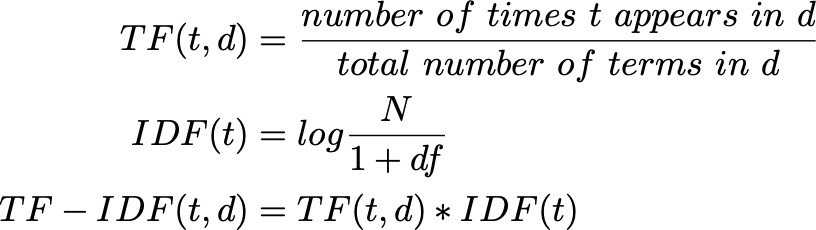
\includegraphics[scale=0.35]{pics/tf_idf}
    \caption{Berechnung von TF-IDF~\cite{tfIdfImage}}
    \label{fig:tf-idf}
\end{figure}

Wenn man diese zwei Werte nun also miteinander multipliziert, erhält man so einen Wert, der indiziert, ob ein Wort relevant für die Bedeutung in dem Dokument ist.
Je höher der Wert ist, desto relevanter ist das Wort sozusagen.

\begin{lstlisting}[label={lst:tf-idf-example},caption={TF-IDF Beispiel}]{TF-IDF Beispiel}
Heute ist ein warmer Tag

Term        Count
Heute       2
ist         1
ein         1
warmer      2
Tag         5
\end{lstlisting}

Bei dem Beispiel ~\ref{lst:tf-idf-example} wird gezeigt, dass die Wörter, die häufig in einem deutschen Satz vorkommen, wie \texttt{ist} oder \texttt{ein}, einen niedrigen Score erhalten und das Wort \texttt{Tag} einen hohen Score aufweist, was bedeutet, dass dieses Wort vermutlich wichtig für die Bedeutung des Satzes ist.

Bei der Text Analysis mit Machine Learning werden solche TF-IDF Algorithmen verwendet, um Daten in Kategorien einzuordnen und wichtige Schlüsselwörter zu extrahieren.
Auch Suchmaschinen wie Google verwenden diese Technologien, um aus dem Suchbegriff des Users die zentrale Aussage herauszufinden und die Suchergebnisse nach ihrer Relevanz zu sortieren.\cite{tfIdf}

\subsection{Word2Vec}
\setauthor{Lukas Starka}

Word2Vec ist das berühmteste Model für Word Embedding.
Unter Word Embedding wird verstanden, dass Texte in denen Wörter dieselbe Bedeutung haben, zusammen repräsentiert werden.
Es werden also sozusagen alle Wörter in einem Koordinatensystem dargestellt, wobei Wörter, die zusammen gehören, nah beieinander sind.
Word2Vec nimmt dabei einen großen Corpus an Text und produziert daraus einen Vektor mit den einzigartigen Wörtern, die ähnlich zueinander sind.
Es ist sehr berühmt dafür, dass demonstriert werden kann, wie Wörter miteinander verbunden sind.

Rasa hat als kleines Nebenprojekt mit \textbf{WhatLies} eine Library geschaffen, die versuchen soll, dass man Word Embeddings besser versteht.
Hierbei kann man Grafiken erstellen, die die Wörter in einem Koordinatensystem repräsentieren.\cite{whatlies}

\begin{figure}[hbt!]
    \centering
    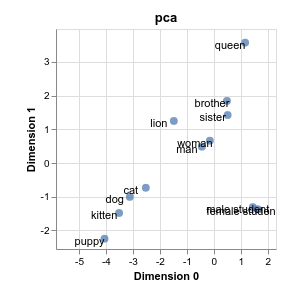
\includegraphics[scale=1]{pics/whatlies_demo}
    \caption{Whatlies Illustration~\cite{whatlies}}
    \label{fig:whatlies-demo}
\end{figure}

Aus der Abbildung ~\ref{fig:whatlies-demo} kann man nun erkennen, dass die Wörter \texttt{brother} und \texttt{sister} oder \texttt{woman} und \texttt{man} nahe beieinander im Raum dargestellt werden.
Außerdem kann man daraus lesen, dass sich \texttt{man} zu \texttt{brother} ähnlich wie \texttt{woman} zu \texttt{sister} oder \texttt{puppy} zu \texttt{dog} sich ähnlich wie \texttt{kitten} zu \texttt{cat} verhält.
Dies findet man dadurch heraus, dass man ein ähnliches Ergebnis bekommt, wenn man die zwei Unterschiede der Vektoren miteinander vergleicht.
Man kann sich außerdem vorstellen, dass man zum Beispiel bei der Rechnung \texttt{King - Man + Woman = ?} als Ergebnis die Position des Wortes \texttt{Queen} erhält.

\subsection{F-Score}\label{F-Score}
\setauthor{Lukas Starka}

Der F-Score wird oft auch als F1-Score oder F-measure bezeichnet und dieser ist ein Maß für die Genauigkeit eines Tests.
Die Formel dafür ist in Abbildung ~\ref{fig:f-score} beschrieben.
In unserem Fall kann man den F-Score beispielsweise verwenden, um zu beschreiben wie oft Intents ~\ref{Intents} richtig klassifiziert wurden.
Die \texttt{precision} gibt dabei an, wie viele Intents richtig klassifiziert wurden, von der Anzahl, wie viele es tatsächlich waren ~\ref{fig:precision}.
Es wird also beispielsweise geschaut, wie viele Intents als \texttt{ask\_htl} identifiziert wurden und, wie viele es tatsächlich sein hätten sollen.
Beim \texttt{recall} ist es auf der anderen Seite so, dass geschaut wird, wie viele Intents richtig klassifiziert wurden und diese Anzahl wird durch die Anzahl, die der Intent vorhergesagt wurde gerechnet.~\ref{fig:recall}.
In unserem Beispiel würde dies bedeuten, dass die Anzahl, wie oft ein Intent tatsächlich \texttt{ask\_htl} war, dividiert durch, wie oft dieser Intent vorhergesagt wurde, wird.
Je näher der insgesamte F-Score dann bei 1 liegt, desto besser ist das Modell und desto besser ist die Genauigkeit.\cite{fScore}

\begin{figure}[hbt!]
    \centering
    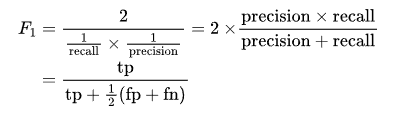
\includegraphics[scale=0.75]{pics/f-score}
    \caption{F-Score Berechnung~\cite{fScore}}
    \label{fig:f-score}
\end{figure}

\begin{figure}[hbt!]
    \centering
    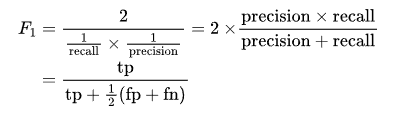
\includegraphics[scale=0.75]{pics/f-score}
    \caption{Precision Berechnung~\cite{precisionRecall}}
    \label{fig:recall}
\end{figure}

\begin{figure}[hbt!]
    \centering
    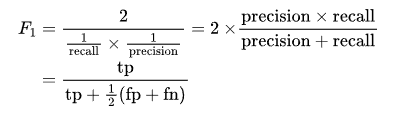
\includegraphics[scale=0.75]{pics/f-score}
    \caption{Recall Berechnung~\cite{precisionRecall}}
    \label{fig:precision}
\end{figure}

\subsection{NLP und NLU Tools}
\setauthor{Lukas Starka}

Ein paar Beispiele für berühmte Tools, die man nützen kann für Natural Language Understanding (NLU) und Natural Language Processing (NLP) sind:

\begin{itemize}
    \item \href{https://www.nltk.org/}{NLTK}: Das Natural Language Toolkit (kurz NLTK) ist wahrscheinlich die berühmteste Python Library für NLP. NLTK besitzt über 50 Ressourcen für das Bearbeiten von Corpora.
    Außerdem gibt es viele eingebaute Libraries für das Analysieren eines Textes, wie die Klassifikation, Tokenization, Stemming, Tagging, Parsing und Semantic Reasoning.
    \item \href{https://spacy.io/}{SpaCy}: SpaCy ist ebenfalls eine sehr berühmte Bibliothek für Python.
    SpaCy beschreibt sich selbst als \texttt{Industrial-Strength Natural Language Processing} und unterstützt über 64 Sprachen.
    SpaCy hat nur einen POS-Tagging-Algorithmus und pro Sprache nur einen Named-Entity-Recognizer, was den Vorteil hat, dass es nicht voller unnötiger Features ist und sich nur auf ein paar wichtige Funktionalitäten konzentriert.
    \item \href{https://www.tensorflow.org/}{TensorFlow}: TensorFlow wird von Google betrieben und ist bei weitem die meist verwendete Library für Deep Learning.
    Außerdem ist die Plattform Open-Source.
    \item \href{https://keras.io/}{Keras}: Keras ist eine Deep Learning Plattform, die in Python geschrieben ist.
    Sie wurde entworfen um schnelle Iterationen und schnelles Ausprobieren mit deep neural networks zu ermöglichen.
    Außerdem bietet Keras ein Interface zu deep neural networks an, welche dann beispielsweise auf TensorFlow, Theano oder anderen Backends laufen können.
    \item \href{https://stanfordnlp.github.io/CoreNLP/}{CoreNLP}: Das CoreNLP Projekt von Stanford ist ein NLP toolkit, welches zwar in Java geschrieben wurde aber auch in anderen Sprachen verwendet werden kann, die auf der JVM Plattform sind.
    \item \href{https://radimrehurek.com/gensim/}{Gensim}: Gensim ist eine Open-Source Library für Python, mit der man semantische NLP Modelle trainieren kann.
    Außerdem ist Gensim Plattform unabhängig und läuft auf jedem Betriebssystem.
    \item \href{https://textblob.readthedocs.io/en/dev/}{TextBlob}: TextBlob ist eine Python Library für das Bearbeiten von Texten.
    \item \href{https://fasttext.cc/}{FastText}: FastText ist eine Open-Source Library, die es Benutzern erlaubt text representations und text classifier zu verwenden.
\end{itemize}


\subsection{NLP in Rasa}
\setauthor{Lukas Starka}

In Rasa kann man sich die verschiedenen Schritte vom Natural Language Processing ansehen, indem man sich die \hyperref[sec:pipeline]{Pipeline} ansieht.
Diese befindet sich in der \textbf{config.yml} Datei und dort sind alle Komponenten aufgelistet, die Rasa verwendet und man kann diese nach Belieben auch selbst bearbeiten.